% Tabela: Resultados do Experimento Gamma
\begin{table}[H]
	\centering
	\caption{Tabela de resultados do Experimento 2.}
		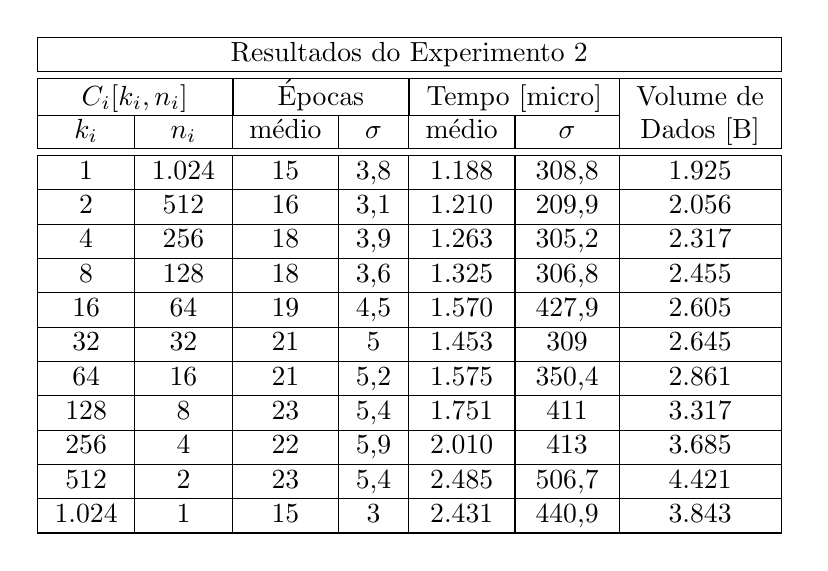
\begin{tikzpicture}
			
		\node[thick, align=center] (table) {
			\begin{tabular}{ |c|c|c|c|c|c|c|c|c|c|c| }
				\hline
				\multicolumn{7}{ |c| }{Resultados do Experimento 2} \\
				\hline \hline
				
				\multicolumn{2}{ |c| }{ $C_i [k_i, n_i]$ } &
				\multicolumn{2}{ |c| }{Épocas} &
				\multicolumn{2}{ |c| }{Tempo [micro]} &
				Volume de \\ \cline{1-6}

				$k_i$ & $n_i$ & médio & $\sigma$ & médio & $\sigma$ & Dados [B]\\
				\hline \hline
				
				1 & 1.024 & 15 & 3,8 & 1.188 & 308,8 & 1.925 \\ \hline
				2 & 512 & 16 & 3,1 & 1.210 & 209,9 & 2.056  \\ \hline
				4 & 256 & 18 & 3,9 & 1.263 & 305,2 & 2.317  \\ \hline
				8 & 128 & 18 & 3,6 & 1.325 & 306,8 & 2.455  \\ \hline
				16 & 64 & 19 & 4,5 & 1.570 & 427,9 & 2.605  \\ \hline
				32 & 32 & 21 & 5 & 1.453 & 309 & 2.645      \\ \hline
				64 & 16 & 21 & 5,2 & 1.575 & 350,4 & 2.861  \\ \hline
				128 & 8 & 23 & 5,4 & 1.751 & 411 & 3.317    \\ \hline
				256 & 4 & 22 & 5,9 & 2.010 & 413 & 3.685    \\ \hline
				512 & 2 & 23 & 5,4 & 2.485 & 506,7 & 4.421  \\ \hline
				1.024 & 1 & 15 & 3 & 2.431 & 440,9 & 3.843   \\ \hline
				
			\end{tabular}
		};

		\end{tikzpicture}
% 	\caption{Tabela de resultados do Experimento 2.}
	\label{tab:resultsGamma}
\end{table}